\chapter{AirTouch}

	\begin{figure}[h]
		\centering
		\subfloat[]{
			\label{fig:animal_family}
			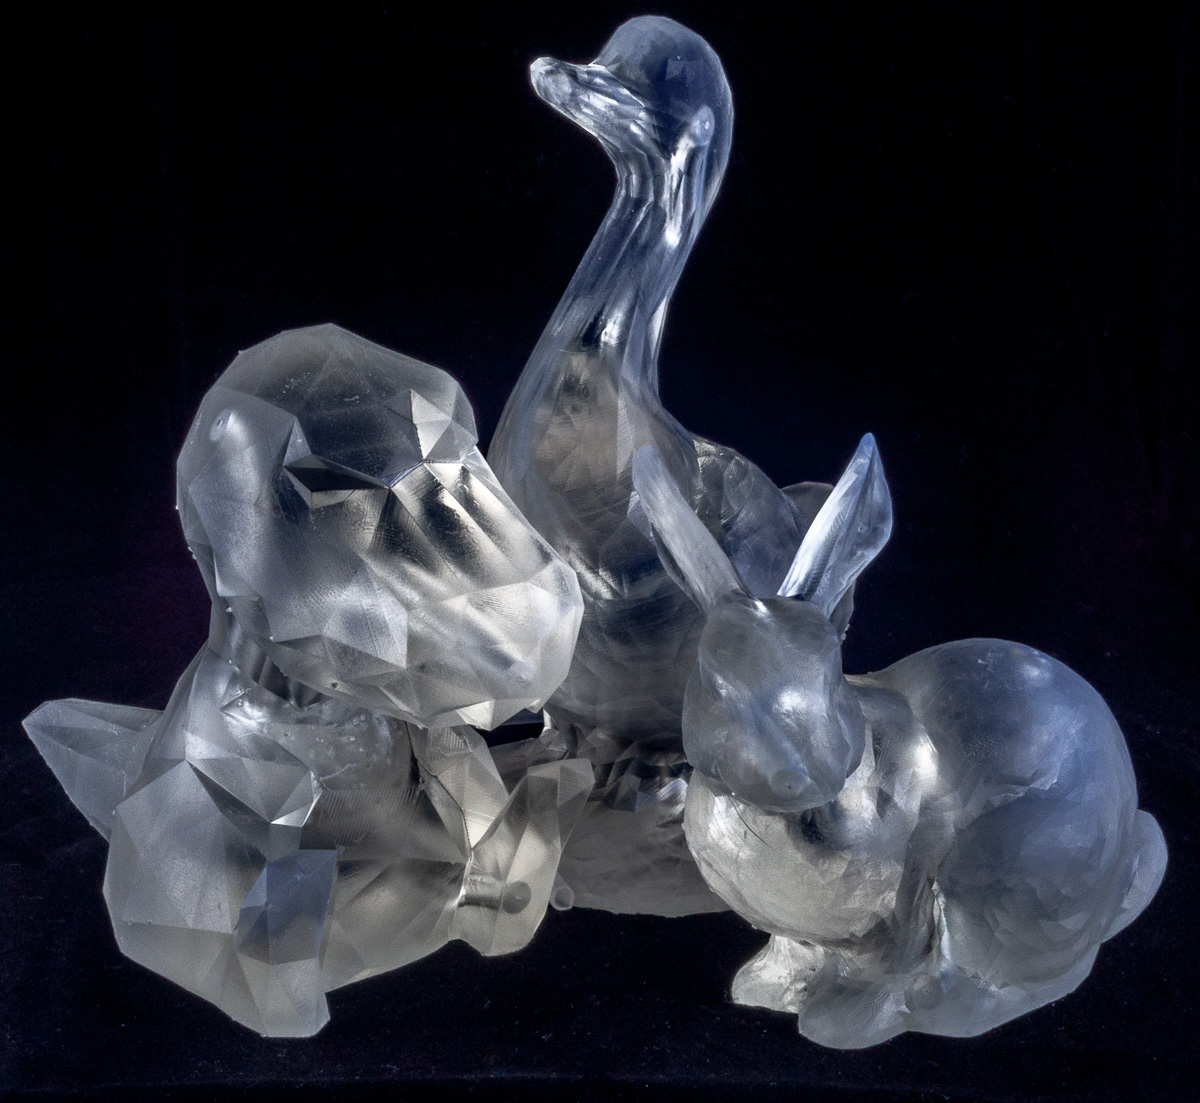
\includegraphics[width=0.33\textwidth]{print-and-play/airtouch/animal_family.jpg}
		}
		\subfloat[]{
			\label{fig:structure}
			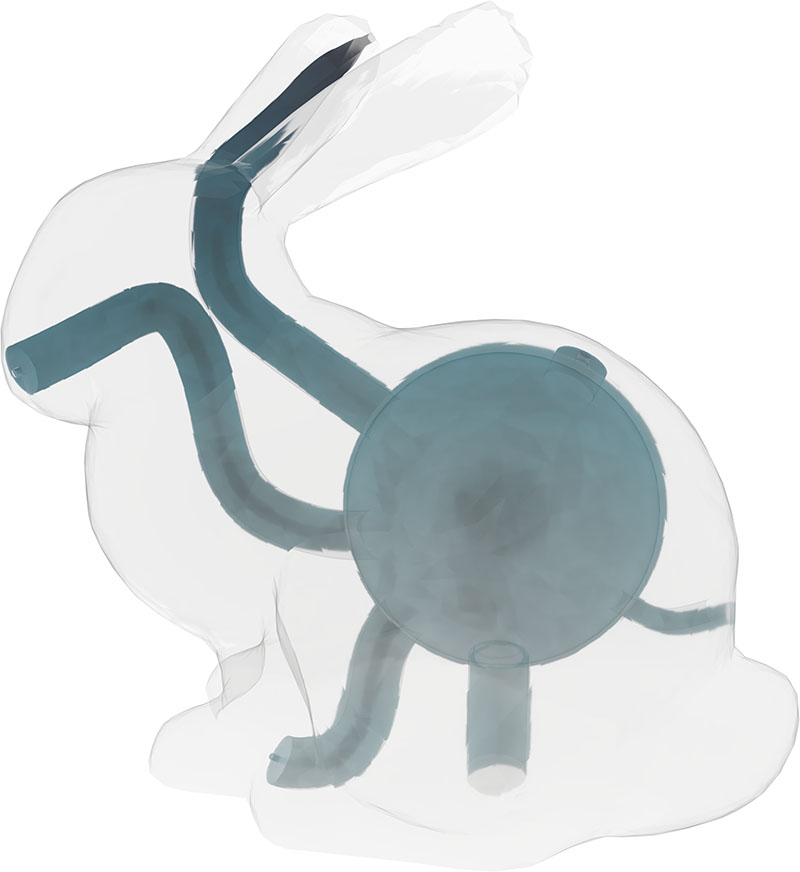
\includegraphics[width=0.33\textwidth]{print-and-play/airtouch/bunny_render.jpg}
		} 
		\subfloat[]{
			\label{fig:touch-bunny}
			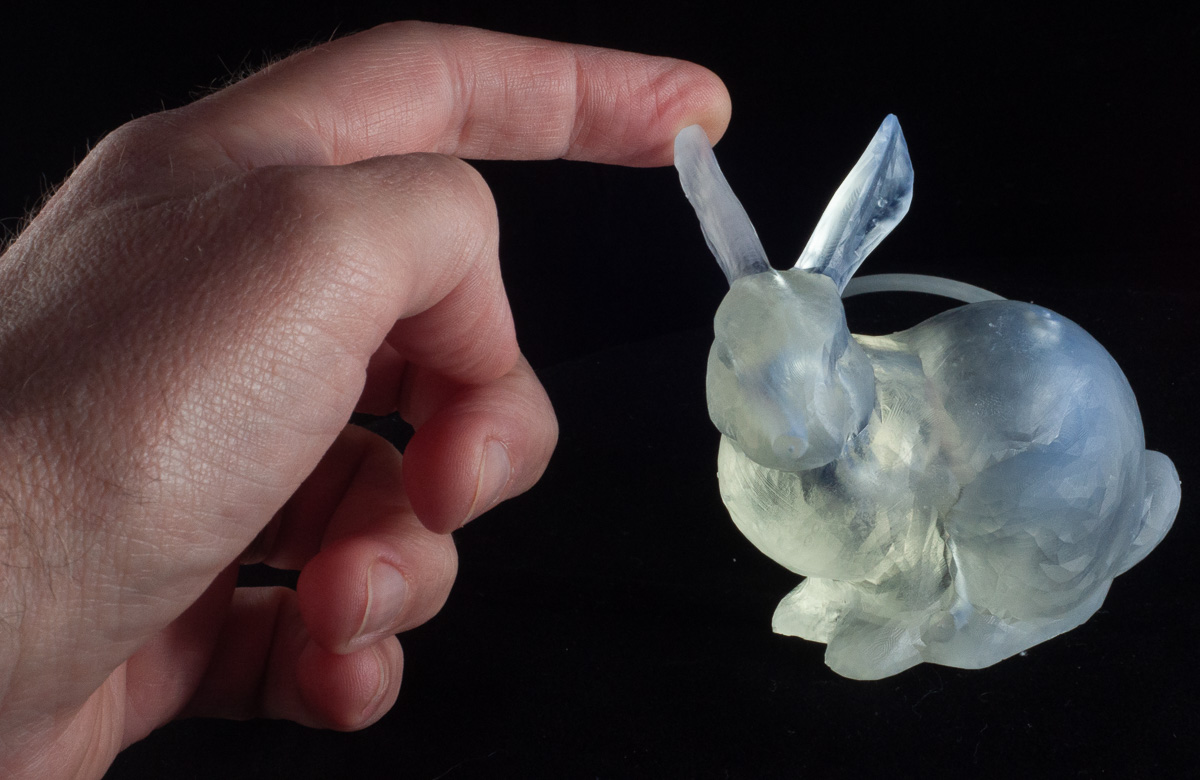
\includegraphics[width=0.33\textwidth]{print-and-play/airtouch/touch-bunny_ear.jpg}
		}
		\label{fig:teaser}

		\caption{\at augments 3D-printed objects to enable touch-sensitivity. It works
			by detecting the pressure change resulting from users blocking tiny air
			outlets fabricated into the objects.}
	\end{figure}

	% Unsure if I should keep the abstract here. It's already in the preface.
	\section*{Abstract}
		3D printing technology can be used to rapidly prototype the look and feel of
		3D objects. However, the objects produced are passive. There has been
		increasing interest in making these objects \emph{interactive}, yet they
		often require assembling components or complex calibration. In this paper,
		we contribute \emph{\at}, a technique that enables designers to fabricate
		touch-sensitive objects with minimal assembly and calibration using
		pneumatic sensing. \at-enabled objects are 3D printed as a single structure
		using a consumer-level 3D printer. \at uses pre-trained machine learning
		models to identify interactions with fabricated objects, meaning that there
		is no calibration required once the object has completed printing. We
		evaluate our technique using fabricated objects with various geometries and
		touch sensitive locations, obtaining accuracies of at least 90\% with 12
		interactive locations.

	\section{Introduction}
		Over the past decade, additive manufacturing has moved from industry to
		desktop-sized 3D printers that empower makers to produce intricate
		three-dimensional shapes. In contrast to this new ease of producing forms,
		making interactive and responsive objects usually requires inserting
		electronic circuitry~\cite{Ramakers:2016, Savage:2015a} and thus requires
		engineering expertise and assembly effort. Similarly to Willis
		\etal~\cite{Willis:2012}, we envision what we call \textit{\pap}: a future
		where interactive objects are ready to use immediately after fabrication,
		without extra effort on the maker's part. Such a capability will empower
		makers, designers, researchers, and educators to instantly turn passive
		fabricated forms into interactive artifacts. While recent research has made
		some progress towards this goal~\cite{Tejada:2018, Schmitz:2019, Ono:2013,
		Shi:2016}, these projects still fall short of being purely \pap: they
		require per-user~\cite{Shi:2016} or per-object~\cite{Tejada:2018,Ono:2013}
		training, are susceptible to environmental
		interference~\cite{Tejada:2018,Shi:2016}, or significantly alter the
		object's external form~\cite{Shi:2016}.

		In this paper, we present \emph{\at}, a novel technique for fabricating
		touch-sensitive objects that are instantly responsive after 3D printing
		without the need for assembly or calibration. Our technique minimally
		modifies the form of the object, adding only a tiny hole to each touch
		location and inlets for an external source of air and a barometric pressure
		sensor; when a user touches a hole, the air pressure inside the object
		changes in a predictable way. \at-enabled objects can be fabricated as a
		single structure on consumer-level resin-based 3D-printers, without the need
		for any post-hoc assembly, and can enable up to 12 different interactive
		locations on fabricated objects.

		To summarize, this work contributes:
		\begin{itemize}
			\item \emph{\at}, a novel technique for fabricating objects that are
				instantly touch-sensitive after printing by measuring differences in air
				pressure inside the object;
			\item a characterization of the number of interactive locations that can
				be enabled with our technique, and its performance; and
			\item a set of applications that demonstrate \at's potential.
		\end{itemize}

	\section{Related Work}
		\at builds on prior research on prototyping and fabricating interactive
		objects, and research around pneumatic interfaces. Earlier in this thesis I
		have presented a comprehensive review of the literature regarding the
		fabrication of interactive objects (see Chapter \ref{ch:background}). This
		section thus presents an overview of previous work on pneumatic interfaces
		that inspired \at.

		\subsection{Pneumatic Input for Interaction}
			\at's use of air pressure as its sensing mechanism is inspired by other
			pneumatic interaction work. A number of projects have used pneumatic
			techniques to augment the digital fabrication process, aiming to reduce
			fabrication time by inflating objects to their final
			form~\cite{Yamaoka:2017, Sareen:2017, Ou:2016}, or to add movement to
			otherwise static objects~\cite{Niiyama:2015, Yao:2013, Niiyama:2015a}.
			
			Various researchers have investigated the use of pressure as an input
			mechanism. Most use sensing of pressure inside flexible enclosures,
			including buttons \cite{Harrison:2009, Vazquez:2015, Gohlke:2016},
			computer mice \cite{Kim:2008}, robots \cite{Slyper:2012}, and balloons
			\cite{Nakajima:2013}. Due to measuring the pressure of air trapped
			inside a flexible structure, these systems are limited to sensing one
			interaction location, and can suffer from ambiguity if the user presses
			with different levels of force. In contrast, \at's use of rigid object
			enables sensing up to 12 different interaction points, and it can operate
			reliably, independent of the user's pressing force on those points.

		\section{\at Overview}
			\begin{figure}[h]
				\centering
				\subfloat[]{
					\label{fig:bunny-no-touches}
					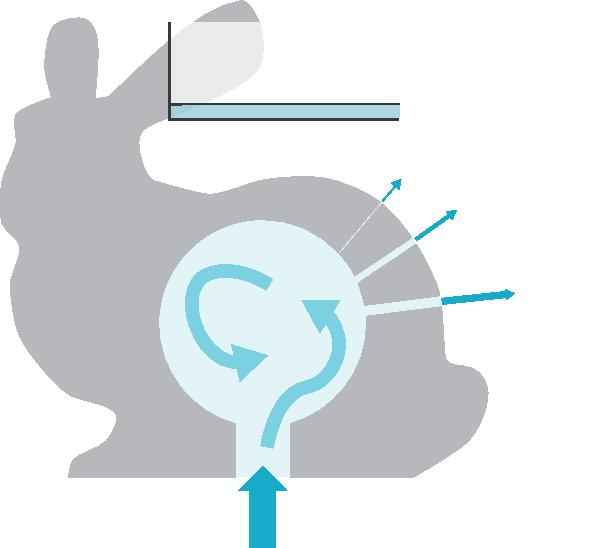
\includegraphics[width=0.33\textwidth]{print-and-play/airtouch/bunny_touches_chamber-page-001.jpg}
				}
				\subfloat[]{
					\label{fig:bunny-touch-1}
					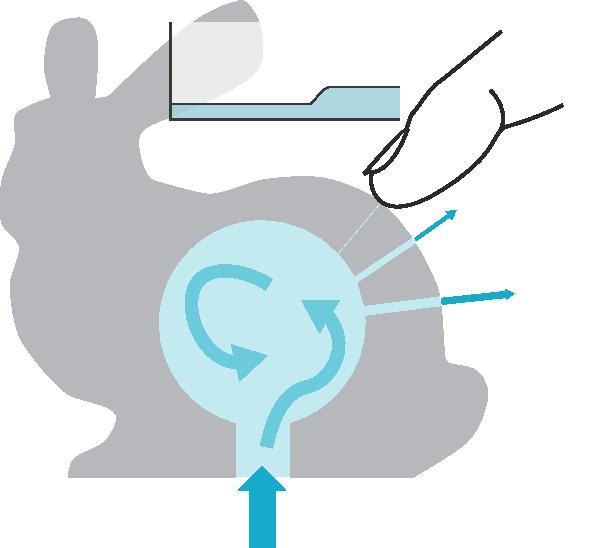
\includegraphics[width=0.33\textwidth]{print-and-play/airtouch/bunny_touches_chamber-page-002.jpg}
				} 
				\subfloat[]{
					\label{fig:bunny-touch-2}
					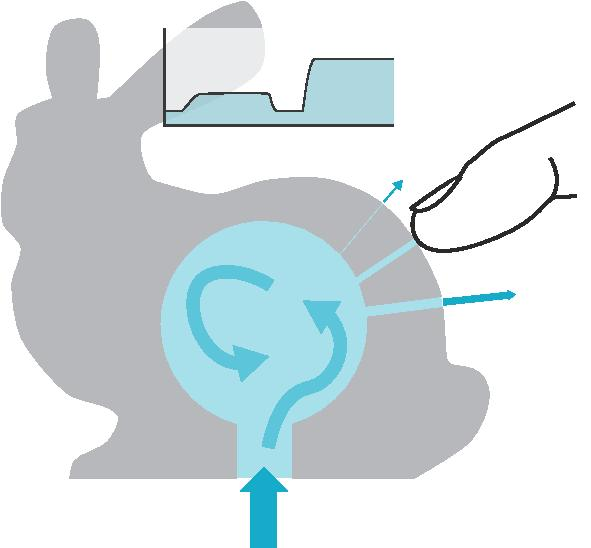
\includegraphics[width=0.33\textwidth]{print-and-play/airtouch/bunny_touches_chamber-page-003.jpg}
				}
				\label{fig:bunny-touches}

				\caption{Representation of \at's working principle. When an outlet is
					covered, the barometric pressure inside the fabricated object rises to an
					identifiable level. As each outlet is unique in size, covering different
					outlets yields a different barometric pressure response.}
			\end{figure}

			\at makes use of some of the basic principles of fluid behavior. In
			particular, we use the \textit{principle of continuity}
			\cite{Rieutord:2015iw}---which indicates that the total flow of air exiting
			an object must equal the flow of air entering the object---and Bernoulli's
			principle \cite{bernoulli1738hydrodynamica}, which relates flow and
			pressure. In combination, these two principles predict that when there is a
			change in the size of an opening through which fluid is passing, the
			pressure will vary in response. Our objects are therefore comprised of a
			series of pressurized tubes with uniquely sized outlets. Covering an outlet
			changes the amount of area through which air can escape, and thereby changes
			the pressure in the object. In the following, we sketch some of the
			mathematical theory of operation that enables \at to function.

			\subsection{Theory of Operation}
				The behavior of \at can be approximated with principles from fluid
				dynamics. By the continuity principle---that the total output from a
				system must be equal to its input---we know that $Q_I$, the flow of air
				entering the object, is equal to $\sum Q_i$, the total flow coming out of
				all openings. The relationship of flow to the cross-sectional area $A$ of
				an opening is given by Bernoulli's principle \cite{Rieutord:2015iw},
				allowing flow to be expressed as

				\begin{equation}
					Q = CA\sqrt{\Delta P}
					\label{eqn:flow}
				\end{equation}

				where $C$ is a constant incorporating an adjustment for the shape of the
				orifice, the density of air, and other unknowns, and $\Delta P$ is the
				difference in pressure before and after the opening. We can now use
				Equation \ref{eqn:flow} to express and simplify the continuity equation in terms
				of the sum of the areas of each outlet $i$ and the difference in pressure
				between the inside of the object and the atmosphere:

				% \begin{align}
				% 	Q_I &= \tsum Q_i \nonumber \\
				% 			&= C\tsum A_i \sqrt{\Delta P}
				% 			\label{eqn:flow-per-outlet}
				% \end{align}

				Now consider the situation where we cover one outlet. Because of
				continuity, the input flow (held constant by the air compressor and
				regulator valve) and output flow are identical to when no outlets are
				blocked. Therefore, the pressure inside the object must increase to
				compensate for the decreased total discharge area. Assuming we have
				blocked outlet $x$, we now have

				% \begin{align}
				% 	C\tsum A_i \sqrt{\Delta P} &= C\left( \tsum A_i - A_x \right) \sqrt{\Delta P_x}
				% 	\label{eqn:pres_touch}
				% \end{align}

				illustrating that with a smaller total area we must have a new, larger
				pressure $\Delta P_x$. Solving Equation \ref{eqn:pres_touch} for $\Delta P_x$
				allows us to predict the new pressure that will result from covering an
				outlet of cross-sectional area $A_x$:

				% \begin{align}
				% 	\Delta P_x =& \frac{(\tsum A_i)^2 \Delta P}{(\tsum A_i - A_x)^2}
				% 	\label{eqn:pressure-from-area}
				% \end{align}

				or, equivalently, given a pressure change of $\Delta P_x$, the outlet area
				which resulted in that pressure change:

				% \begin{align}
				% 	A_x = \tsum A_i \left(1 - \sqrt{\frac{\Delta P}{\Delta P_x}} \right)
				% 	\label{eqn:area-from-pressure}
				% \end{align}
				
				As presented here, these fluid dynamics equations work with
				incompressible, steady flows---that is, liquids flowing in steady
				state---and perfectly shaped outlets of known geometry. Our system does
				not hold to these constraints: 3D-printed objects, and thereby our
				outlets, are not perfect; air is compressible; and our objects are subject
				to internal turbulence due to their complex geometry (see
				Figure \ref{fig:structure}). Due to these factors, the above equations do not
				perfectly match our observed data, but provide guidelines for
				understanding and predicting the general behavior of the system.

			\subsection{Internal Structure}
				\at adds an internal structure to 3D models that distribute incoming flow
				from an air compressor to outlets on the object's surface
				(Figure \ref{fig:structure}). This internal structure consists of several
				components: a central flow-distribution chamber which supplies all tubes
				with air; an inlet via which the air source provides pressurized air flow
				to the flow-distribution chamber; a connection point for the pressure
				sensor; a series of tubes that connect the flow-distribution chamber to
				touch locations on the object's surface. By using this structure in all
				\at-augmented objects, we ensure that the pressure increases when touching
				the same outlet are comparable, regardless to the outer geometry of the
				augmented object.

			\subsection{Sensing User Interactions}
				The basic user interaction with an \at-enabled object is via touch. When a
				user touches one of the outlets on the object's surface, the airflow
				through that outlet is blocked. As each outlet has a different size, the
				airflow through each outlet is unique and is proportional to the outlet
				area (Equation \ref{eqn:flow-per-outlet}). Blocking the flow from an outlet causes
				a identifiable rise in the barometric pressure inside the object. Our
				system records these changes in air pressure using a barometric sensor,
				and translates them to an outlet ID, and subsequent position on the
				object's surface. Figure \ref{fig:bunny-touches} shows an abstract
				representation of the unique barometric increases sensed when the user
				covers different outlets, and Figure \ref{fig:bar-touches} shows actual sensed
				touch data.

    \section{Parameter Exploration}
			Every \at object contains a flow-distribution chamber, tubes, and outlets.
			In this section, we report on the design and fabrication of this internal
			structure based on literature and additional testing. Our design decisions
			were guided by the following three requirements: (1) the object, including
			the internal structure, must be fabricatable with a consumer-level 3D
			printers; (2) the outside geometry of the object cannot be modified; (3)
			per-object calibration is not allowed.

			\begin{figure}
				\centering
					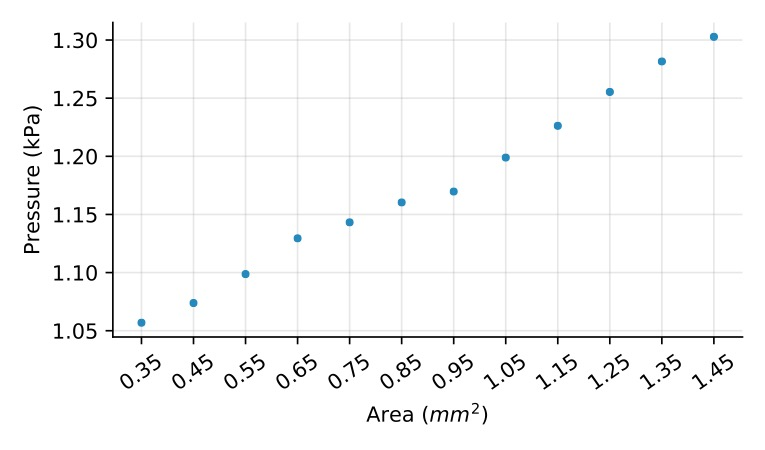
\includegraphics[trim={0 0.5cm 0 0},clip,width=\columnwidth]{print-and-play/airtouch/plot-touches.jpg}
					\caption{Pressure in kilopascals (kPa) for single touches on twelve
						differently sized outlets (ranging in cross-sectional area from
						.35\,mm$^2$ to 1.45\,mm$^2$ in 0.1\,mm$^2$ increments).}
					\label{fig:bar-touches}
			\end{figure}

			\subsection{Experimental Setup}
				We constructed a test setup consisting of a JunAir 2000-40PD air
				compressor, Festo MS4-LR-1/4-D5-AS valve, and an analog Panasonic PS-A
				(ADP5) barometric sensor. The sensor is connected to an Arduino Uno,
				which samples the air pressure at 5\,kHz. We connect standard air
				compressor tubing (polyethylene, 6\,mm diameter) to the valve, and the
				barometric sensor to the object. This sensor is responsible for
				detecting the subtle pressure changes in the system caused by user
				interactions, and can sense pressures relative to atmospheric pressure
				from 0 to 6 kiloPascals (kPa). The sensor's limited operating range
				requires that we empirically set the valve's value for objects having a
				different number of outlets to avoid saturation. To reduce the noise
				from the sensor readings, we filter the incoming signal using the
				1\texteuro~Filter~\cite{Casiez:2012} using $\beta$ and cutoff values
				set empirically, dependent on the base pressure output of the
				compressor.
					
				We print our objects using the FormLabs Form~2 3D~printer, a
				consumer-level resin-based stereolithography (STL) printer capable of
				high resolutions. We use STL technology because in our initial
				experiments, it became clear that current FDM-based printers are not
				capable of precisely printing tiny holes at arbitrary orientations. We
				print \at-enabled objects as single structures with no assembly needed.
				The only addition to the standard post-processing required of all STL
				print processes is a 30-second flushing stage with the air compressor
				immediately after printing to prevent residual resin causing blockages
				during curing.

			\subsection{Flow-Distribution Chamber}
				\at objects embed a spherical flow distribution chamber to distribute
				incoming flow between between tubes; 3D printing small-size spherical
				shapes does not require support material. Instead of using a flow
				distribution chamber, we also experimented with hollowing the object. In
				these shell structures, outlets are simply holes and do not require
				tubes. This approach, however, requires per-object touch calibration
				while also requiring higher pressures for operation, as the air flows
				through the entire geometry of the object. In contrast, the spherical
				flow-distribution chamber has the same shape across objects and ensures
				a consistent airflow. To allow touch interactivity on small objects with
				\at, the flow-distribution chamber should be small to fit objects of
				various geometries. Therefore, we fabricated three Stanford bunnies,
				each with identical outlet configurations but with varying
				flow-distribution chamber diameters of 15, 20 and 30\,mm in diameter. We
				recorded the barometric pressure changes when covering the outlets and
				found that the volume of the chamber does not significantly impact the
				relative pressure variations between outlets. We did find, however, that
				smaller cavities yield a higher noise profile on the resulting signals;
				therefore, as a compromise between size and performance, we used
				flow-distribution chambers of 30\,mm diameter in most of our further
				experiments.

			\subsection{Tubes}
		    The touch locations on the object's surface are connected to the
		    flow-distribution chamber with cylindrical tubes. To allow tubes to be
		    embedded in small objects, we want the diameter to be as small as
		    possible. After experimenting with different diameters, we picked 5\,mm
		    tubes as the best tradeoff between size and printability. While 3\,mm
		    tubes often worked, we found that with this smaller size it was
		    difficult to guarantee that all of the resin would drain from the tubes
		    before post-print curing.
		    
		    Based on fluid dynamics literature~\cite{Brown:2002it}, we determined
		    that the length of the tube as well as the area of the outlet influences
		    the barometric pressure inside the object. First, we tested if varying
		    the tube length produces enough difference in barometric pressure to
		    identify the tube from which the airflow is blocked. To do so, we
		    fabricated three objects of varying geometries: a duck, a bunny and a
		    CHI-nosaur. Each has a 30\,mm-diameter chamber and four outlets, placed
		    at the foot (.35\,mm$^2$), nose/beak (.65\,mm$^2$), ear (.95\,mm$^2$),
		    and back (1.25\,mm$^2$). Although these objects share the same cavity
		    size and outlet configuration, their interior tube lengths vary between
		    3--100\,mm. Figure \ref{fig:tube-lengths} shows no significant
		    difference in pressure responses when covering each of the outlets for
		    all three objects. In the next section, we report on testing the impact
		    of varying the area of the outlet.
		    
		    \begin{figure}
					\centering
					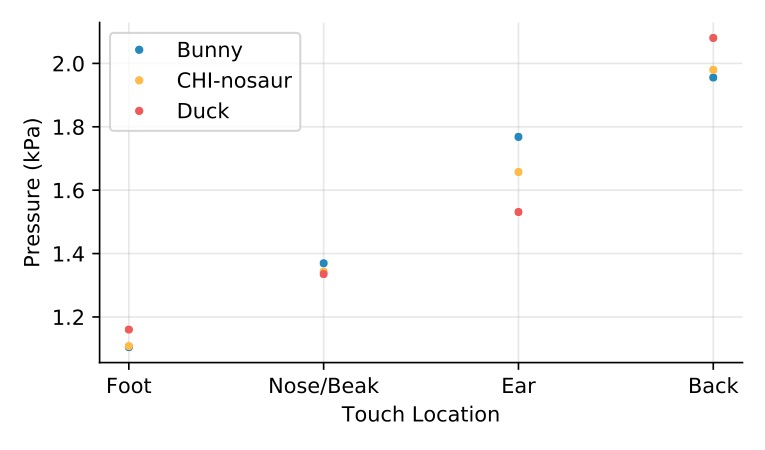
\includegraphics[width=.90\textwidth]{print-and-play/airtouch/bunny-dino-duck-comparison.jpeg}
					\caption{Pressure results by location on interactive animals. Note
						that the pressure difference between animal models is significantly
						smaller than the difference between touches on outlets of different
						sizes.}
					\label{fig:tube-lengths}
		    \end{figure}

		    \begin{figure}[h]
					\centering
					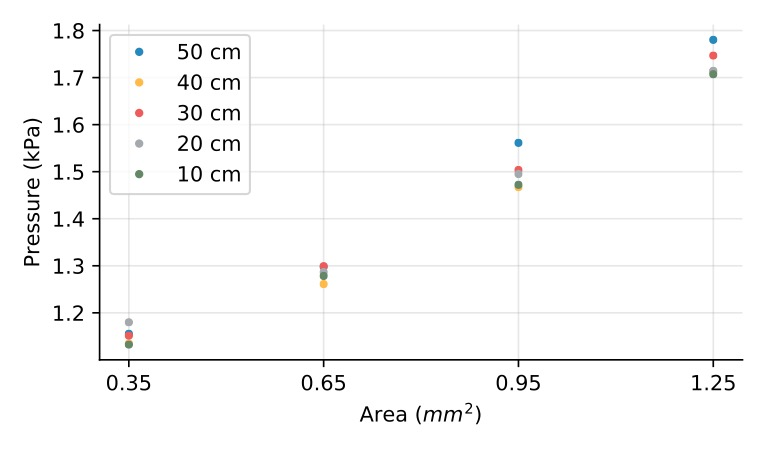
\includegraphics[width=.90\columnwidth]{print-and-play/airtouch/tube-lengths.jpg}
					\caption{Pressure results by tube length. Note that the pressure
						difference between tube lengths is significantly smaller than the
						difference between touches on outlets of different sizes.}
					\label{fig:tube-lengths}
		    \end{figure}
		    
		    Although we did not find significant difference between the pressure
		    increases from interacting with desktop-sized objects of different
		    geometries, we wished to identify the potential size limits of our
		    technique. Because our available printers are limited in size, we used
		    6\,mm polyethelyne (PE) tubing (hardness: Shore~D~52) to simulate
		    printed channels. We fabricated a standalone flow-distribution chamber
		    of 30\,mm diameter with four 6\,mm outlets. We also fabricated four
		    6\,mm tube caps with outlets of the same sizes as the animals listed
		    above. We connected one 50\,cm length of tube to each outlet,
		    terminating each with one cap, and recorded the pressure for each. We
		    repeated this procedure four more times, shortening the tube length by
		    10\,cm each time. Figure \ref{fig:tube-lengths} illustrates our results: we
		    see very little impact of tube length on pressure. As an additional
		    informal experiment, we connected one outlet to a 40\,m-long tube. At
		    this length, the volume of air in the tube is significant (2\,L) and is
		    subject to both compression and losses due to friction
		    \cite{Brown:2002it}. Due to these effects we see a noticeable
		    2--3-second delay for the pressure to reach its full amplitude. While
		    not suitable for interactions requiring immediate responsiveness, this
		    example shows the versatility and scalability of our technique. Although
		    these experiments suggests that \at is capable of augmenting larger
		    objects, more experimentation is still needed.
		    
			\subsection{Outlets}
				In contrast to varying the length of the tubes, we did observe a
				significant difference in the barometric pressure response when blocking
				the airflow from tubes having different outlet diameters. To minimally
				disturb the object's original geometry and ensure outlets are always
				covered entirely when touched, we wanted to use outlets with diameters
				as small as possible. During our initial exploration phase, we found
				that our printer was unreliable in printing outlets smaller than 0.6\,mm
				in diameter. Additionally, we observed that the difference between
				barometric pressure responses of small outlets are not significant in
				the presence of large outlets. Therefore, we empirically set the maximum
				outlet diameter to 1.50\,mm.
            
				With an operational range of 0.6--1.50\,mm for outlet diameters, we
				optimized the step size between outlet diameters to maximize the number
				of outlets while ensuring significant differences between barometric
				pressure responses from all outlets. Equation
				\ref{eqn:area-from-pressure} indicates that the pressure/area
				relationship is nearly linear for our range of diameters. We printed
				three test objects, each with outlets in the operational diameter range
				but with area steps of 0.02, 0.06, and 0.1\,mm$^2$ between subsequent
				outlets. We then connected each to the testing setup and recorded
				touches on each outlet. We found that with the smaller area increments,
				the pressure change between neighboring outlet sizes was insufficient to
				offer a clear separation in the presence of sensor noise (approximately
				0.01 kPa). Therefore, all of our subsequent objets are printed with at
				least a 0.1\,mm$^2$ separation between hole areas. Table
				\ref{tab:hole-sizes} illustrates, at actual size, the final set of 12
				outlet dimensions we use.
            
				As discussed earlier, the tubes connecting the outlets to the chamber
				are 5\,mm in diameter to prevent clogging. We therefore reduce the last
				1\,mm of the tube to form the outlet, as shown in Figure
				\ref{fig:tube-reduction}.        

				% \newcommand{\ccc}[1]{ \begin{tikzpicture} \fill[black] (0,0) circle [radius=#1mm]; \end{tikzpicture}}
				% \begin{table}[]
				% 	\centering
				% 	\newcolumntype{C}{>{\centering\scriptsize\arraybackslash}X}
				% 	\begin{tabularx}{\columnwidth}{CCCCCCCCCCCC}
				% 			\ccc{0.334} & \ccc{0.378} & \ccc{0.418} & \ccc{0.455} & \ccc{0.489} & \ccc{0.52} & \ccc{0.55} & \ccc{0.578} & \ccc{0.605} & \ccc{0.631} & \ccc{0.656} & \ccc{0.679} \\
				% 			0.334 & 0.378 & 0.418 & 0.455 & 0.489 & 0.52 & 0.55 & 0.578 & 0.605 & 0.631 & 0.656 & 0.679 \\
				% 	\end{tabularx} 
				% 	\caption{Final outlet dimensions shown at actual size with radius in
				% 		millimeters indicated under each. The area increases by .1\,mm$^2$
				% 		between each subsequent hole, ranging between 0.35--1.45\,mm$^2$.}
				% 	\label{tab:hole-sizes}
				% \end{table}

    		\begin{figure}
    			\centering
    			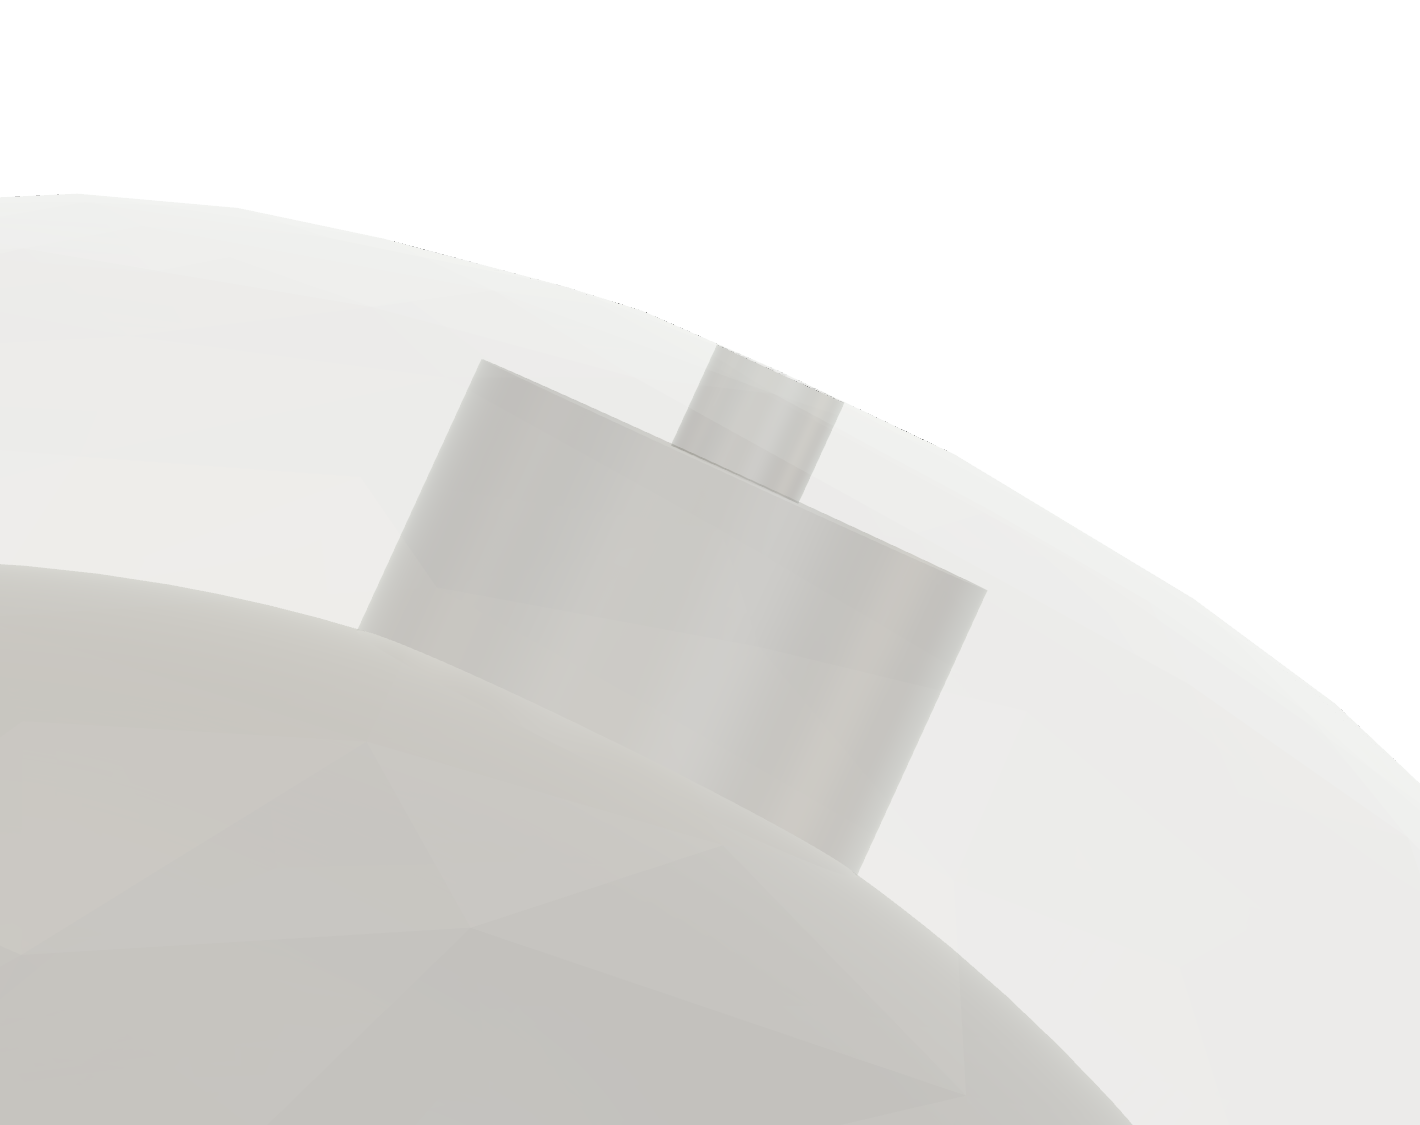
\includegraphics[width=.65\linewidth]{print-and-play/airtouch/tube-closeup}
    			\caption{Close up view of the connection between the tube and the
						outlet.}
    			\label{fig:tube-reduction}
    		\end{figure}

	\section{Software}
		In this section, we discuss the algorithms for recognizing and identifying
		touches as well as the software implementation that facilitates designing
		AirTouch's internal tube structure.

		\subsection{Designing \at Objects}
			\at-enabled objects require an object's internal structure to be augmented
			with an inlet for pressurized air, a flow-distribution chamber, uniquely
			sized outlets at desired touch locations, and a connection for the sensor.
			To facilitate designing \at objects, we created an Autodesk Meshmixer
			script which automatically modifies the model's internal structure and
			adds appropriately-sized outlets to objects at user-selected locations.
			Our script embeds a flow-distribution chamber inside the model, and uses
			the tube routing algorithm described in \cite{Savage:2014} to attach a
			tube spanning from the cavity to locations selected by the designer. If
			more precision is necessary, tubes can be added manually to objects using
			standard CAD software.

		\subsection{Touch Recognition and Identification}
			In order to identify when an outlet is covered, we first segment the
			signal coming from the sensor into 100-sample windows. We then calculate
			the mean and standard deviation for each window, and once the standard
			deviation surpasses an empirically set threshold, we assume there has been
			a touch or release event. To identify whether this change has been a touch
			or a release, we compare the mean of the current window with the mean of
			the previous one: if the current mean is higher than the previous, an
			outlet has been covered; if not, an outlet has been released.
					
			Once we have determined that a touch event has happened, we identify which
			outlet has been covered. We take the mean of the 1000 samples previous to
			the touch event as the pressure baseline, and divide it by the mean of the
			1000 samples following the touch. This ratio compensates for drift in the
			signal caused by minor atmospheric fluctuations and imprecisions in the
			regulator valve.

    \section{Performance Testing}
			To show the viability of \at, we evaluated our recognition pipeline on a
			set of \at-enabled objects of varying geometries and outlet
			configurations: an interactive bar chart, a Stanford bunny, a color hue
			selector and a dual-touch sensing sphere.  For each outlet configuration,
			we train a machine learning model (SVM with rbf kernel) using a single
			instance consisting of mean and standard deviation for the registered
			pressures for a given touch. We proceed to cycle through the outlets of
			each object, recording the classification result for each touch. We repeat
			this process four times per object.
        
			\begin{figure}[h]
				\centering
				\subfloat[]{
					\label{fig:bar-plot-confusion}
					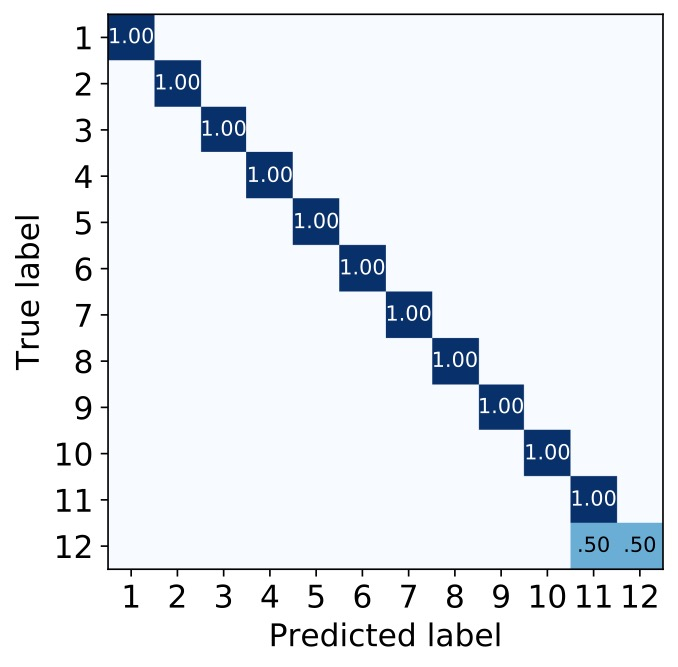
\includegraphics[width=.43\textwidth]{print-and-play/airtouch/barchart-confusion.jpg}
				}
				\subfloat[]{
					\label{fig:bunny-confusion}
					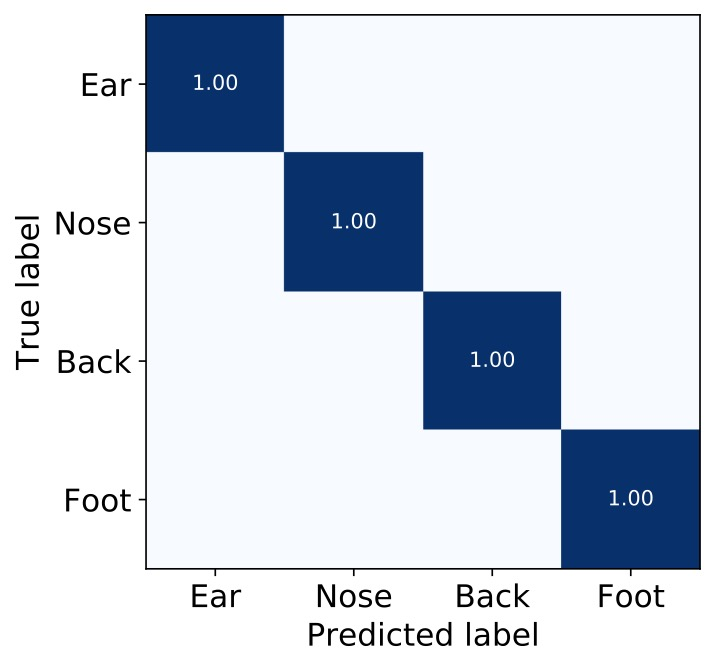
\includegraphics[width=.43\textwidth]{print-and-play/airtouch/bunny-conf.jpg}
				} \hfill
				\subfloat[]{
					\label{fig:color-picker-confusion}
					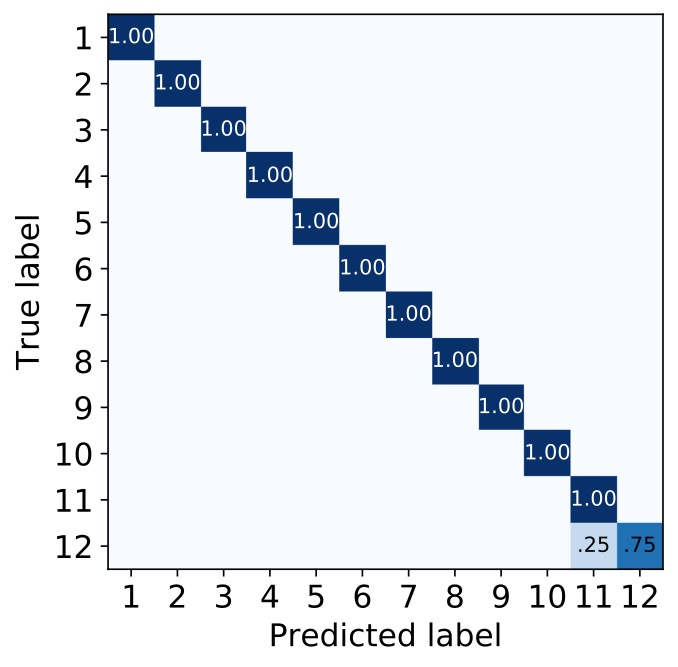
\includegraphics[width=.43\textwidth]{print-and-play/airtouch/color.jpg}
				}
				\subfloat[]{
					\label{fig:grasp-sensing-sphere-confusion}
					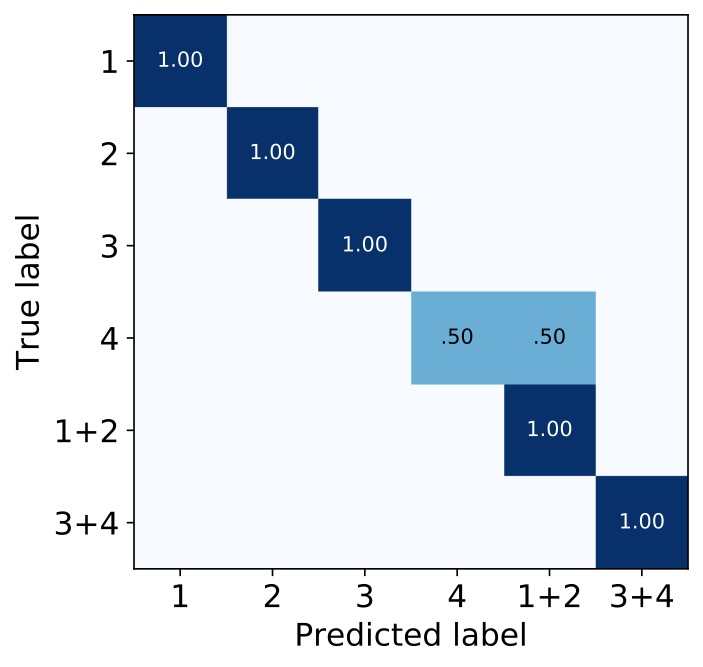
\includegraphics[width=.43\textwidth]{print-and-play/airtouch/grasping.jpg}
				}

				\caption{Confusion matrices of classification accuracies from our tests:
					interactive bar plot (a); augmented Stanford bunny (b); color hue
					selector (c); grasp-sensing sphere (d). Each cell indicates the number
					of classified touch interactions to a predicted class (row) for each
					actual class (column).}
				\label{fig:confusion-matrices}%
			\end{figure}

			We obtained average accuracies of 95.5\% (for the bar chart), 100\%
			(Stanford bunny), 97.75\% (color hue selector), and 91.6\% (Grasp sensing
			cube). Figure \ref{fig:confusion-matrices} shows a detailed view of the
			performance for each object.

			\begin{figure*}[h]
				\centering
				\subfloat[]{
				\label{fig:app_1}
				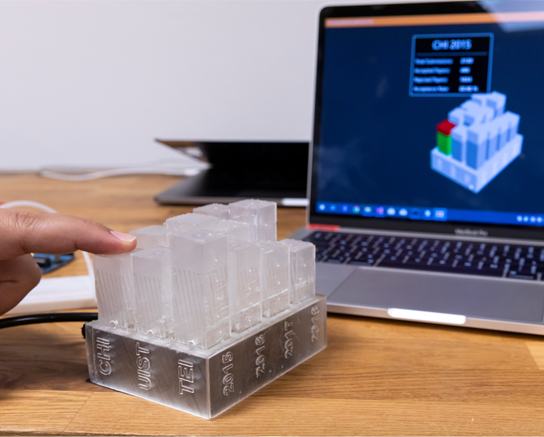
\includegraphics[width=.43\textwidth]{print-and-play/airtouch/Applications_Barchart.png}
				}
				\subfloat[]{
				\label{fig:app_2}
				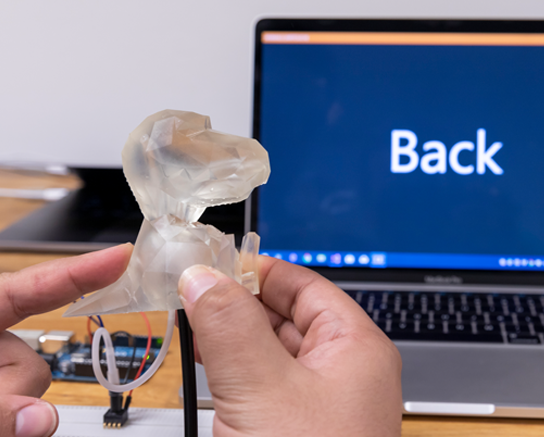
\includegraphics[width=.43\textwidth]{print-and-play/airtouch/Applications_Animal.png}
				} \hfill
				\subfloat[]{
				\label{fig:app_3}
				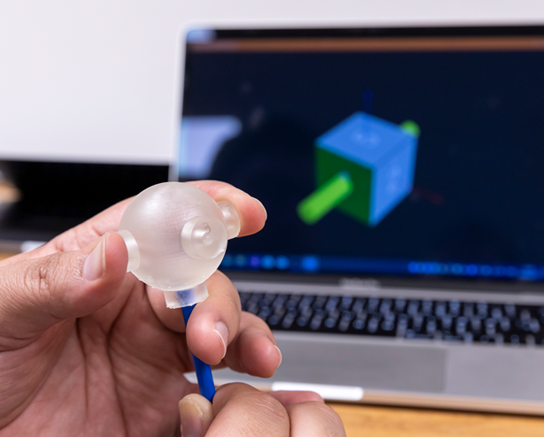
\includegraphics[width=.43\textwidth]{print-and-play/airtouch/Applications_Grasping.png}
				}
				\subfloat[]{
				\label{fig:app_4}
				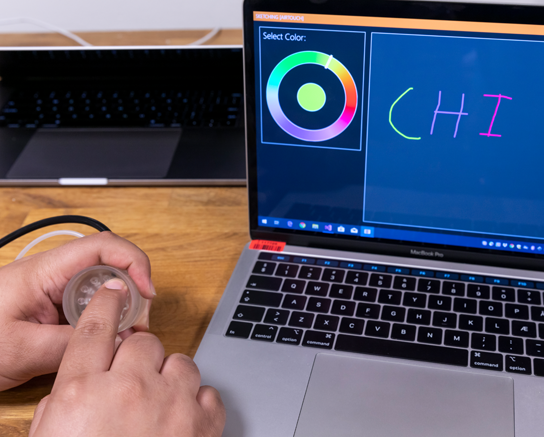
\includegraphics[width=.43\textwidth]{print-and-play/airtouch/Applications_ColorDial.png}
				}
				\caption{Example \at Applications. With \at, interactive objects are
					fabricated as a single structure without any post-print assembly or
					calibration. We showcase objects of different geometries augmented with
					\at: an interactive bar chart (a); interactive animals (b);
					grasp-sensing sphere (c); and a color hue selector (d).}
				\label{fig:apps}
			\end{figure*}

	\section{Example Designs and Applications}
		Because its ease of fabrication, and large number of interactive locations,
		\at lends itself to the rapid prototyping of interactive devices. Below we
		present a number of example usages of \at which illustrate its potential.
		All applications are developed in C\# and WPF and receive data (over a
		socket connection) from Python code running the touch detection described
		above.
		
		\subsection{Interactive 3D Bar Chart}
			Recent work has highlighted the benefits of data
			physicalization~\cite{Jansen:2015cu}. We designed a three-dimensional bar
			plot displaying the relation between the submitted and accepted papers in
			the past four years to CHI, UIST, and TEI (Figure
			\ref{fig:barchart,fig:app_1}).  To obtain more information about the
			proceedings, the user touches the top of a bar, and the companion
			application shows the acceptance rate, number of accepted papers for the
			year and conference in question.
		    
		\subsection{Interactive Animals}
			\at can identify interactions on objects of varying geometries, but with
			the same outlet configurations, with a single, pre-trained machine
			learning model. We fabricated a set of interactive animals of different
			outer geometries, but sharing the same outlet configuration (i.e., an
			ear of different animals has the same outlet diameter). We augmented a
			Stanford bunny, a duck, and a CHI-nosaur with interactive locations on
			the nose, ear, back and leg. When a location is touched, the
			corresponding label is displayed (Figure \ref{fig:app_2}).
		    
		\subsection{Grasp Sensing}
			To showcase \at's dual-touch sensing capabilities, we developed a
			touch-sensing sphere (Figure \ref{fig:app_3}). We augmented a sphere with
			four touch locations throughout its surface. When an outlet is covered,
			the companion application highlights which face is touched. When two
			outlets are covered simultaneously, the system highlights both faces.
		    
		\subsection{Color Hue Selector}
			\at can enable up to 12 interactive locations on 3D-printed objects. We
			designed a circular color hue selector for a drawing application (Figure
			\ref{fig:app_4}). The user selects a color using the selector, and sketch
			in the drawing window.
		    
	\section{Discussions and Limitations}
		While \at is successful in fabricating touch-sensitive objects and tangible
		input components without the need of any post-print assembly it has
		limitations. The most obvious one is the need for an air compressor to power
		the fabricated objects. Although we employed an air compressor to power our
		fabricated objects, other air sources might be used, granted they guarantee
		a constant stream of air. A miniature air pump, similar to the one used by
		V\'azquez and collaborators in~\cite{Vazquez:2015dm}, can power \at-enabled
		objects given their low pressure requirements.
		
		Another limitation of our technique is that it's only able to augment
		objects fabricated using high-resolution 3D-printing technologies. We
		explored fabricating \at-enabled objects using Fused Deposition Modeling
		(FDM) printers, but encountered a number of issues. Because of its
		layer-by-layer fabrication procedure, some objects fabricated with our
		Lulzbot Taz~6 and QiDi Technology X-One presented significant leaks in the
		internal structure of the object, hindering the technique's performance. We
		plan to explore the effects of employing smoothing techniques (e.g., acetone
		smoothing), and varying the shell thickness of the model when printing to
		reduce leaks. FDM printers also lack the precision of STL printers, meaning
		that when printing outlets. Future work can explore the different approaches
		to ensure the correct fabrication of outlet sizes on lower resolution
		equipment.
		
		Although we experienced a noticeable latency in our 40m-long tube
		experiments between when covering the outlet and the signal reaching its
		full amplitude, these effects were not present in \at-enabled objects---the
		pressure increase upon covering an outlet was instant. Future work can
		explore the use of our technique to enable richer gestures such as swiping
		and sliding on fabricated objects.
		
		Employing the same principle used to detect individual touches, \at can
		identify up to two simultaneous touches on different locations throughout
		the fabricated object. Because the increase in pressure is proportional to
		the outlet area, covering multiple outlets can be identified as a new touch
		location---as long as the sum of the areas of the covered outlets results in
		a unique change in pressure. In order to guarantee a 0.1\,mm$^2$ separation
		between the outlets and their respective combinations, we used outlets sizes
		of 0.4\,mm$^2$, 0.5\,mm$^2$, 0.6\,mm$^2$, and 0.8\,mm$^2$ in our test
		objects.
		
		Finally, we experienced small variations in the measured barometric
		pressures inside our fabricated objects when compared to previous days. This
		is due to the everyday changes in environmental barometric pressure. To
		evaluate the effects of these everyday changes in our system's performance
		we performed a preliminary test over a period of four consecutive days where
		the ambient pressure varied from 0.1 to 0.7 kPa. Using the bunny model, we
		recorded touches each day and found that the pressure variation shifted the
		baseline of the measurements by an amount smaller than the separation
		between different touches.
	    
	\section{Conclusion}
		In this paper we introduced \at: a technique for fabricating touch-sensitive
		objects without the need of any post-print activities such as assembly or
		calibration. We presented the theory behind \at, our explorations of
		parameters for both interaction and successful fabrication, and guidelines
		for designing \at-enabled objects. We illustrated \at's flexibility with
		several applications, and showed that \at is able to identify interactions
		with accuracies of at least 91\% with 12 interactive locations.
	
	% \section{Acknowledgements}
	% 	We wish to thank Prof. Larry Villasmil from the Rochester Institute of
	% 	Technology for his valuable input, and Mengyu Zhong for her help designing
	% 	and fabricating test objects.